
\noindent
Real world network topologies often have assymmetric, lossy links. In order to 
evaluate the performance of the Reachback Firefly Algorithm (RFA) on such topologies, we
have conducted a number of experiments with link level loss on the TinyOS sensor
network simulator. This paper gives details of these experiments and draws conclusions
from the results attained. \newline

\subsection{Experimental Setup}

\noindent
In this paper we examine the impact of different levels of link level loss on a regular GRID topology.
In particular, we explore the impact of different levels of bidirectional 
link level loss on a 4x4 regular grid topology with 16 nodes and 24 bidirectional links.  
Each experiment is run for 3600 seconds and is repeated 10 times with different random seeds.
The results reported in the graphs represent averages and standard deviations. 
The firing function constant (FFC) value is kept constant at 100 for all simulations
since most simulations achieved synchronicity with this FFC value.
\newline

\noindent
On TOSSIM, loss is specified via a \emph{.nss} file that is essentially a topology file that contains 
information on the loss on a link from every node in the network to every other node. 
It is important to note that this topology remains fixed during the course of a simulation.
The \emph{.nss} file allows the specification of assymetric link loss since it requires the specification of loss 
on a link from node A to node B as well as from node B to node A.
The default implementation of loss in TOSSIM interprets the loss values in the topology file as \emph{bit-level}
loss. We modified this implementation to interpret the loss values in the topology files as \emph{packet-level}
loss. Details of these code changes are provided in the appendix at the end of this document.
In our implementation a loss value of 0 means a perfect link and a loss value of 1 means a broken link. 
{\bf A loss value of 0.9 signifies that on every link there is a 90\% chance of a packet being dropped}. \newline

\noindent
In our experiments, we introduce loss in a {\it flood-fill} manner in a 4x4 grid. 
Fig.~\ref{fig:graph1-6} shows how loss is gradually introduced in the network. After
loss is added to 4 links, node 6 is not guaranteed to always receive information from
any of its neighbors. Fig.~\ref{fig:graph6-12}-\ref{fig:graph24} show the order
in which loss is introduced from 6 to all 24 links in the topology. 
The number of lossy links is varied at the beginning of each experiment and kept
constant for the duration of that experiment.
\newline

\begin{figure}
\centerline{%
\includegraphics[width=14cm,angle=0]{figures/lossGraph1-6.eps}
}
\caption{{\it Grid topology: From no links with loss to 6 links with loss. All loss is bidirectional. The numbers on the links indicate the order in which loss is introduced. This is consistent in Fig.~\ref{fig:graph6-12}-\ref{fig:graph24}.}}.
\label{fig:graph1-6}
\end{figure}

\begin{figure}
\centerline{%
\includegraphics[width=14cm,angle=0]{figures/lossGraph6-12.eps}
}
\caption{ {\it Grid topology: From 6 links with loss to 12 links with loss.}}
\label{fig:graph6-12}
\end{figure}


\begin{figure}
\centerline{%
\includegraphics[width=14cm,angle=0]{figures/lossGraph12-20.eps}
}
\caption{ {\it Grid topology: From 12 links with loss to 20 links with loss.}}
\label{fig:graph12-20}
\end{figure}


\begin{figure}
\centerline{%
\includegraphics[width=5cm,angle=0]{figures/lossGraph24.eps}
}
\caption{{\it Grid topology: All 24 links have loss.}}
\label{fig:graph24}
\end{figure}

\subsection{Results}

\noindent
Fig.~\ref{fig:linkloss0.1}-\ref{fig:linkloss0.9} show how synchronicity is affected when the 
loss per link is varied from 0.1 to 0.5 to 0.9 respectively. 
The error bars show the standard deviation computed over 10 different simulations.
The time to sync metric defined in~\ref{} represents the speed at which synchronicity is 
attained and the group spread metrics, also defined in ~\ref{},
represents the tightness of the synchronicity.  In particular, the 50th percentile group spread 
represents the tightness of synchronicity of 50\% of the groups (clusters of node firings) 
after synchronicity is achieved.
Fig.~\ref{fig:percent-synch-loss} shows the percentage of cases that synchronized for
each of these levels of loss. This percentage represents the number of 
experiments that achieved synchronicity for a given value of loss on a given number of links
as a fraction of the the total number of runs carried out with these settings. The total execution 
time of each simulation is 3600 seconds.  Due to the nature of the implementation of our time to sync
metric, we do not count any experiment with more than 1500 seconds of time to sync as one that
achieved synchronicity.  
\newline


\begin{figure}
\centerline{%
\includegraphics[width=14cm]{figures/percent-synch-linkloss.eps}
}
\caption{ {\it Percentage of cases that synchronized when the link level loss is varied from 0.1 to 0.5 to 0.9 in a grid topology.  Experiments with link level loss of 0.1 always achieved synchronicity.  Experiments with link level loss of 0.9 on more than 8 links achieved synchronicity less than 50\% of the time.}}
\label{fig:percent-synch-loss}
\end{figure}

\begin{table}[t]
\begin{center}
\begin{tabular}{|c|c|c|c|c|c|c|} \hline
Amount of Loss & Max TTS (sec) & Min TTS (sec) & Max GS-50 (ms) & Min GS-50 (ms) & Max GS-90 (ms) & Min GS-90 (ms) \\ \hline \hline
0.1            &  393.53     &  135.84       &  9.959      &  6.035    &   46.72    & 8.391  \\ 
0.5            &  554.92     &  137.88       &  37.553     &  6.116    &   91.415   & 8.586  \\
0.9            &  *          &  166.04       &  62.664     &  6.349    &   96.626   & 8.660  \\
\hline \hline
\end{tabular}
\end{center}
\caption{{\it Range of variation of time to sync and group spread when link loss is varied. For a given amount of loss, the max and min values are taken over experiments in which the number of links with that of loss is varied from 1 to 24.  Values are reported for experiments that achieved synchronicity in at least half of their runs.  The max TTS for the 0.9 loss experiments is omitted since many of its runs did not converge especially for large numbers of lossy links.}}
\label{table:maxMin}
\end{table}

\begin{figure}
\centerline{%
(a)
\includegraphics[width=6cm,angle=270]{figures/TTSvsLossyLinks0.1.ps}
(b)
\includegraphics[width=6cm,angle=270]{figures/GSvsLossyLinks0.1.ps}
}
\caption{{\it Impact of link level loss when the loss probability is 0.1. {\bf(a)} Time to sync: Initially the addition of four or more lossy links cause the nodes to take longer to converge.  After 10 lossy links, however, the system begins to converge more quickly as more lossy links are added. {\bf (b)} Group Spread: For 50\% of the groups the tightness of synchronicity does not vary significantly as more lossy links are added.  This is also confirmed by the numbers in Table~\ref{table:maxMin}.  For 90\% of the groups the spread does increase initially as 4 or more lossy links are added but consistently decreases after more than 16 lossy links are added.}}
\label{fig:linkloss0.1}
\end{figure}

\begin{figure}
\centerline{%
(a)
\includegraphics[width=6cm,angle=270]{figures/TTSvsLossyLinks0.5.ps}
(b)
\includegraphics[width=6cm,angle=270]{figures/GSvsLossyLinks0.5.ps}
}
\caption{ {\it Impact of link level loss when the loss probability is 0.5. {\bf (a)} Time to sync: Initially the addition of four or more lossy links cause the nodes to take longer to converge.  After 10 lossy links, the time taken for the system to converge sometimes drops although this trend is not consistent.  {\bf (b)} Group Spread: For both 50\% and 90\% of the groups thetightness of synchronicity initially decreases (group spread increases) after 6 or more lossy links are added but this begins to consistently decrease as 20 or more lossy links are added. Table~\ref{table:maxMin} shows that 80\% of the experiments with 20 or more links with loss probabilities of 0.5 converged: therefore, these results are fairly reliable. The error bars on the 24 lossy links indicate that the group spreads for all the runs for this experiment are lower than those for 20 lossy links.  The group spread graph also shows that there is a large jump in the group spread of 90\% of the groups after loss is added to 4 links (and thus node 6 has a chance of losing messages from all its neighbors), and this value dramatically decreases when all 24 links in the entire system are lossy.}}
\label{fig:linkloss0.5}
\end{figure}

\begin{figure}
\centerline{%
(a)
\includegraphics[width=6cm,angle=270]{figures/TTSvsLossyLinks0.9.ps}
(b)
\includegraphics[width=6cm,angle=270]{figures/GSvsLossyLinks0.9.ps}
}
\caption{ {\it Impact of link level loss when the loss probability is 0.9.  Fig.~\ref{fig:percent-synch-loss} shows that after adding 8 links with loss probabilities of 0.9, less than 50\% of the runs for these experiments converged.  Therefore, after 8 lossy links or so, the metric values for these experiments are unreliable. {\bf (a)} Time to Sync: Up to the addition of 6 lossy links, the network takes longer to converge as more lossy links are added. {\bf (b)} Group Spread: 50\% and 90\% of the groups take longer to converge up to this point as more lossy links are added. The graph also shows the same sharp increase in group spread in 90\% of the groups when 4 lossy links are added that was observed in Fig.~\ref{fig:linkloss0.5}.}}
\label{fig:linkloss0.9}
\end{figure}


\subsection{Discussion and Analysis}
Table~\ref{table:maxMin} confirms a basic hypothesis that time to sync and group spread both increase as the probability
of loss is increased from 0.1 to 0.5. Since more messages are likely to be lost, nodes are likely to miss firings
that allow them to increment their position on their firing functions and therefore there is greater liklihood for them
to stay out of sync, and to take longer to get upto sync with each other.  Also, the tightness of the synchronicity
achieved deteriorates as the link level loss gets higher.
Since, as Fig~\ref{fig:percent-synch-loss} shows, that at least 80\% of 
the runs for these experiments converged, we can be fairly confident of these results.  The fact that many of 
the experiments for link loss of 0.9 did not converge is also not surprising since one would expect it to be 
more difficult for the system to reach convergence when nodes have a 90\% chance of losing packets from their neighbors.  \newline

\noindent
Interesting patterns in the data emerge as we examine how the quality and speed of synchronicity is influenced 
by the number of lossy links added to the network. In all the experiments, the time to sync and group spread 
rises sharply when there are 4 lossy links in the network. This jump is proportional to the loss probability
used in the experiment.
Fig.~\ref{fig:graph1-6} shows that the first 4 lossy links emanate
from node 6. Thus one could conclude that synchronicity suffers significantly when a particular node in the network 
has all lossy links.
The degree to which time to sync and group spread increase is proportional to the level of loss on the links. The 
higher the loss probability the higher the surge in the two metrics. \newline

\noindent
The graphs also show that the group spread and time to sync do not rise consistently as more lossy links
are introduced in the network.  In fact, there are fluctations in group spread and time to sync as the
number of lossy links increases above 10 links in all of the experiments.  In particular the time to sync and
group spread when all 24 links are lossy in the network are lower than when there are fewer (for instance 6) lossy links
in the network.  This is true for the experiments regardles of the amount of loss probability.  
This is rather surprising since one would expect that if all links in the network 
are lossy, all the nodes in the network are likely to receive fewer firing messages from their neighbors
and are therefore likely to converge more slowly and achieve less tight convergence as a result of having
lost important firing messages.
In order to explore this trend, it is important to focus on the results for loss probabilities 
of 0.1 and 0.5 since at least 80\% runs for these experiments converged and therefore 
these results are comparatively more reliable than the ones with loss probability of 0.9.
In the 0.1 loss probability experiments, one way to explore the reasons behind this trend is look 
at the phase plots of nodes in the 10 lossy links experiments versus those of nodes in the 16 lossy links 
experiments. The time to sync with 10 lossy links is much higher than with 16 lossy links in thise case.
On the other hand the 90th percentile group spread with 10 lossy links is lower than that
with 16 lossy links.  The comparatively high error bar on the group spread of the 16 lossy link experiment indicates that 
there could be considerable variation in that value. \newpage

\begin{figure*}
\centerline{%
(a)
\includegraphics[width=6cm,angle=270]{figures/10-links-loss-0.1-run-10-begin-phase.ps}
(b)
\includegraphics[width=6cm,angle=270]{figures/16-links-loss-0.1-run-10-begin-phase.ps}
}
\caption{ {\it Initial phase plots of nodes in a {\bf(a)} 10 lossy link experiment and {\bf(b)} 16 lossy link experiment when the the loss probability is 0.1.}}
\label{fig:begin-phase10-16}
\end{figure*}


\begin{figure}
\centerline{%
(a)
\includegraphics[width=6cm,angle=270]{figures/10-links-loss-0.1-run-10-phase.ps}
(b)
\includegraphics[width=6cm,angle=270]{figures/16-links-loss-0.1-run-10-phase.ps}
}
\caption{ {\it {\bf (a)} Phase plot of Fig~\ref{fig:begin-phase10-16}(a) between a time period of 700-1000 seconds during which the nodes reach convergence to synchrony.  {\bf (b)} A zoomed in view of Fig~\ref{fig:begin-phase10-16}(b) showing
the different synchronized subgroups just before they merge into one synchronized group.}
In (a) individual nodes 6,9 and 10 are out of phase with the remaining nodes. In (b) there are three distinct synchronized subgroups that gradually converge to synchrony.}
\label{fig:phase10-16}
\end{figure}

\noindent
Fig~\ref{fig:begin-phase10-16}(a) and \ref{fig:phase10-16}(a) show that in the 10 lossy link experiment, right before synchronicity is achieved,
several individual nodes are out of phase with a large synchronized group of nodes. These nodes are nodes 6, 9 and 10, and the
topology graphs in Fig~\ref{fig:graph6-12} show that the lossy links introduced in the topology for this experiment, are connected to these nodes, and essentially all the links connecting these nodes are lossy.
Fig~\ref{fig:begin-phase10-16}(b) and \ref{fig:phase10-16}(b) show that there are several synchronized subgroups
in the 16 lossy link experiment that merge to form one synchronized group. Fig~\ref{fig:phase10-16}(b) shows that
the three main subgroups are of nodes: (12,13), (2,3,6,7,10,11,14,15) and (0,1,4,5,8).
Examining the topology graphs in Fig~\ref{fig:graph1-6}-\ref{fig:graph24}
show that the nodes in these synchronized subgroups are adjacent to each other and connected by lossy links. 
Overall the two phase plots indicate that if synchronized subgroups form early on, then the system reaches synchrony
faster than when several individual nodes are out of phase with the rest of the system. \newline

\noindent
To further explore this hypothesis, it could be helpful to examine the phase plots of nodes in the 0.5 loss probability
experiments.
In particular, the experiments for 10 lossy links and 24 lossy links serve as interesting candidates.
The time to sync and 50th and 90th percentile group spread of the 10 lossy link experiment is higher
than that of the 24 lossy link experiment.  
Fig.~\ref{fig:begin-phase10-24}(a) and (b) show the phase plots for these experiments.
Indeed as our hypothesis predicts, several synchronized subgroups merge
to form one synchronized group for the 24 lossy links experiment.  Fig.~\ref{fig:phase24}, a zoomed in view of the 24 lossy
link experiment, shows that the subgroups consist of nodes: (4,0,8), (10,11,12,13,14,15) and (1,2,3,5,6,7,9).  
For the 10 lossy link experiment node 10 as well as 
a subgroup of nodes (6,9) remain completely out of phase with the remaining nodes for more than 200 seconds.  
Therefore, these phase plots for the 0.5 loss probability experiments also indicate that when the majority of
links in the system are lossy, it is easier for synchronized subgroups to form and these subgroups merge to attain synchrony
faster than individual out-of-phase nodes would.   \newline

\noindent
The group spread of the 24 lossy link experiment is also lower than that of the 10 lossy link experiment, indicating
that the synchronized subgroups in the 24 lossy link experiment merge to form tighter synchronicity than the individual 
nodes attain when they merge in the 10 lossy link experiment. The group spread values in the previous phase plots
of the 0.1 loss probability experiments do not support this hypothesis however, since in those plots the 90th 
percentile group spread of the 16 lossy link experiment is higher than that of the 10 lossy link
experiment. The high error bars on the 16 lossy link experiment however motivate us to examine more plots in order 
to evaluate our hypothesis about the group spread.
While the plots are not shown here, we examined the phase plots of nodes in the 20 lossy link experiment when the 
loss probability is 0.5 and compared this with the phase plot of the 24 lossy link experiment with the same loss 
probability.  The phase plot for the 20 lossy link experiment shows a number of individual out of phase nodes
consisting of nodes 0,1,2,4,5,8, 10,and 13 that merge simultaneously with two remaining synchronized subgroups
to attain complete synchronicity.  Since the 20 lossy link experiment has higher group spread and time to sync
than the 24 lossy link experiment, the phase plot confirms our hypothesis that individual out of sync nodes
lengthen the time taken to achieve synchronicity and decrease the tightness of the synchronicity achieved.
Examination of the phase plot of the 16 lossy link experiment for 0.5 loss probability also confirms this hypothesis. \newline

\noindent
The magnitude of the phase differerences between the synchronized subgroups is also interesting. 
Fig.~\ref{fig:begin-phase10-16}(b) and Fig~\ref{fig:begin-phase10-24}(b) show that the phase differences
between the synchronized subgroups decrease steadily whereas the phase plots of the individual out of sync
nodes in Fig.~\ref{fig:begin-phase10-16}(a) and Fig~\ref{fig:begin-phase10-24}(a) show that their phase
differences remain constant until they suddenly merge towards synchrony.  This observation shows that it is
more likely for at least one member in a synchronized subgroup to detect a firing than for a single out of sync
node when the links in the network are lossy.  This could be one of the reasons why the emergence of synchronized
subgroups leads to faster and tighter synchronicity.

\begin{figure}
\centerline{%
(a)
\includegraphics[width=6cm,angle=270]{figures/10-links-loss-0.5-run-6-begin-phase.ps}
(b)
\includegraphics[width=6cm,angle=270]{figures/24-links-loss-0.5-run-6-begin-phase.ps}
}
\caption{ {\it Initial phase plots of nodes in a {\bf(a)} 10 lossy link experiment and {\bf(b)} 24 lossy link experiment when the loss probability is 0.5.}. In (a) node 10 is significantly out of phase with the remaining two synchronized subgroups. In (b), there are three main synchronized subgroups that gradually converge to synchrony with the others.}
\label{fig:begin-phase10-24}
\end{figure}

\begin{figure}
\centerline{%
\includegraphics[width=6cm,angle=270]{figures/24-links-loss-0.5-run-6-phase.ps}
}
\caption{ {\it A zoomed in view of Fig~\ref{fig:begin-phase10-24}(b) showing
the different synchronized subgroups just before they merge into one synchronized group.}}
\label{fig:phase24}
\end{figure}

\subsection{Conclusions}

The lossy link experiments lead us to make two main observations. First the magnitude of loss probability 
in the network significantly
impacts the quality and speed of synchronicity. The lower the probability of loss, the greater the chances for 
the network to attain faster and tighter synchronicity. Secondly, more lossy links do not necessarily imply
worse synchronicity.  In fact, if there are many lossy links in the network, the chances of clusters of
synchronized nodes forming are higher, and these clusters of synchronized nodes merge faster to attain
tighter synchronicity than individual out of sync nodes would.

%%% End
\newpage

